\section{Problem 4}

This problem consists in the analysis of the scattering parameters for a common-emitter amplifier with BC549 as seen in figure \ref{p3:bc549}.

\begin{figure}[H] 
\centering
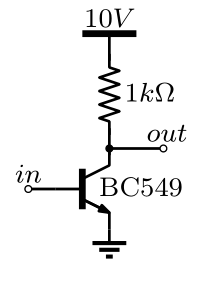
\includegraphics[width=3.5cm]{images/bc549.png}
\caption{Common-emitter amplifier with a bipolar junction transistor BC549.}
\label{p3:bc549} 
\end{figure}

The circuit above was simulated via ADS with the conditions below:

\begin{itemize}
    \item BJT polarized with $675 mV$;
    \item Source and load impedance of $Z_L = Z_S = 50 \Omega$;
    \item S-parameters simulation with frequency sweep between $1 kHz$ and $1 GHz$;
\end{itemize}

The ADS allow us to plot the behavior of each one of the scattering parameters considering 2 ports as seen in figure \ref{p4:sparams}.

\begin{figure}[H] 
\centering
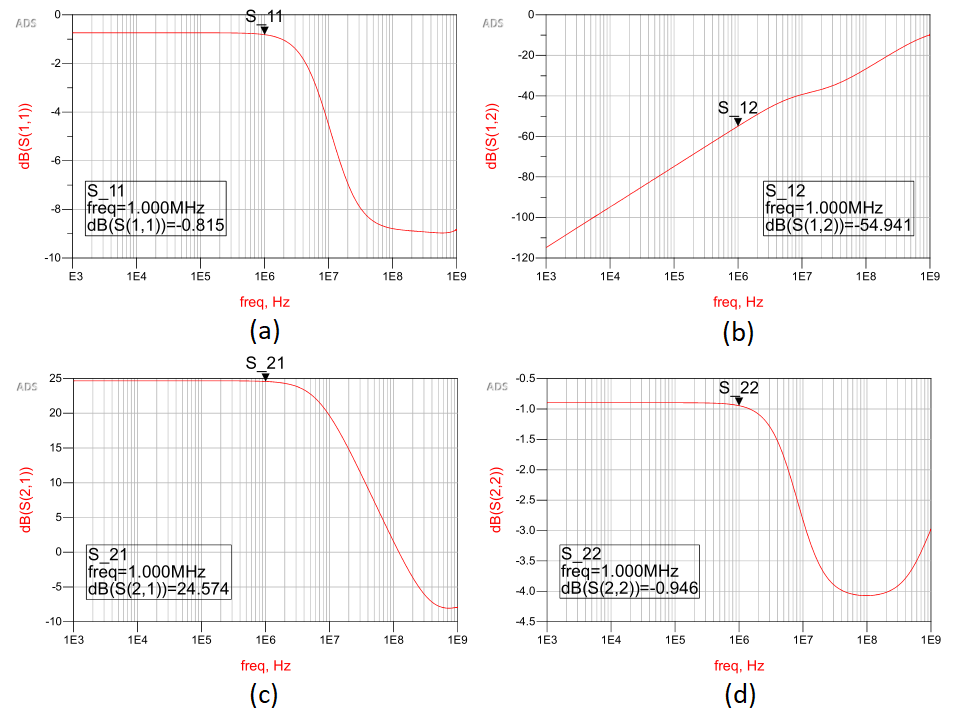
\includegraphics[width=15cm]{images/sparams.png}
\caption{Common-emitter amplifier with BC549 scattering parameters magnitude: (a) $s_{11}$, (b) $s_{12}$, (c) $s_{21}$ and (d) $s_{22}$.}
\label{p4:sparams} 
\end{figure}

Regarding the parameters $s_{11}$ and $s_{22}$ that denote the reflection coefficient in each port, we can observe by its magnitudes that they exert an approximately constant influence (but different between them) until the frequency of $1 MHz$. For higher frequencies the values tend to reduce, meaning that the reflected waves with these frequencies will be less influential. Regarding the other parameters their behavior are quiet different. The magnitude of $s_{21}$ (portion of the available power at the source [port 1] that was actually delivered to the load [port 2]) keeps approximately constant until $1 MHz$ and then drops. The behavior of $s_{11}$ and $s_{22}$ beyond $1 MHz$ are acceptable, but the effort is meaningless because of $s_{21}$, meaning that the reflected power is reduced as the transmitted power too. 

Once the circuit is not symmetrical, all the parameters will differ. The parameter $s_{12}$ have the oddest behavior, because it keeps risen but with no significant magnitude, meaning that the power flow from collector to base is nearly null but will rise due to the leakage current from the semiconductor junction reversed biased.

\subsection{Transducer power gain vs. Power gain}

The standard power gain is the relation between the output power (load power) with the input power $G_P = P_L/P_{in}$. But this relation does not take into account the power related to the reflected wave in the input port. So another metric is the transducer power gain the relates the output power with the total power available at the source $G_T = P_L/P_{av,s}$. So this allow us to analyse the maximum power gain at a impedance match situation.

Considering that the load power is $P_L = P_{av,s} \times |s_{21}|^2$ it is clear to see that the transducer power gain is simply the equation \ref{p4:gt}. Once the input power will be the available power at the source deducted the reflection losses: $P_{in} = P_{av,s} - P_r$. The power reflected at port 1 is $P_r = P_{av,s} \times |s_{11}|^2$. Replacing the reflected power and the available power as a function of $P_{av,s} = P_L / |s_{21}|^2$ we obtain a expression that depends only on the scattering parameters for the power gain in the equation \ref{p4:gp}. The expression also shows that in a condition without reflection ($s_{11} = 0$) both the gains are equals.

\begin{equation} \label{p4:gt}
    G_T = \frac{P_L}{P_{av,s}} = |s_{21}|^2
\end{equation}

\begin{equation} \label{p4:gp}
    G_P = \frac{P_L}{P_{in}} = \frac{|s_{21}|^2}{1 - |s_{11}|^2}
\end{equation}

In the previous simulation with load and source impedance of $50 \Omega$ and frequency of $100 MHz$, we can see by the plot of figure \ref{p4:gpgt} that $G_P = 1.648$ and $G_T = 1.43$. Since $s_{11}$ is lower than the unit for each and all frequencies of the plot, it results in $G_P > G_T$ and this is a coherent result because $P_{av,s} > P_{in}$, remembering that the available power incorporates the input power and the losses.


\begin{figure}[H] 
\centering
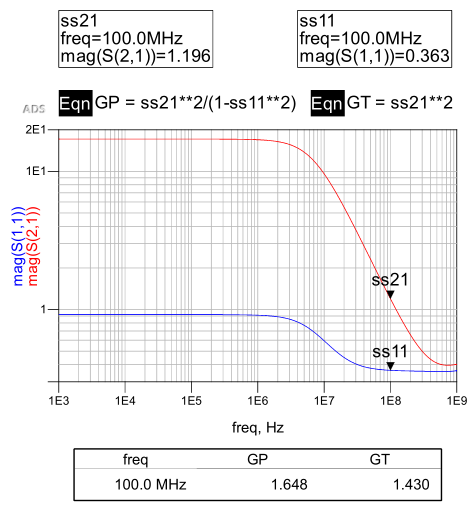
\includegraphics[width=9cm]{images/gpgt.png}
\caption{Common-emitter amplifier with BC549 transducer power gain ($G_T$) and power gain ($G_P$) at $100 MHz$.}
\label{p4:gpgt} 
\end{figure}

A practical way to prove this result is to feed the amplifier with a sine voltage of $1 mV_p$ and $100 MHz$ (same conditions of load and source impedance, polarization and transistor model) and check the power values. According to figure \ref{p4:gtproof} the resulting gain is $G_T = 1.395$. It differs from the previous result because the latter was found by a transient simulation with a limited time step that reduces precision and has convergence problems and the other was found via a simulation of S-parameters in a single point of frequency.

\begin{figure}[H] 
\centering
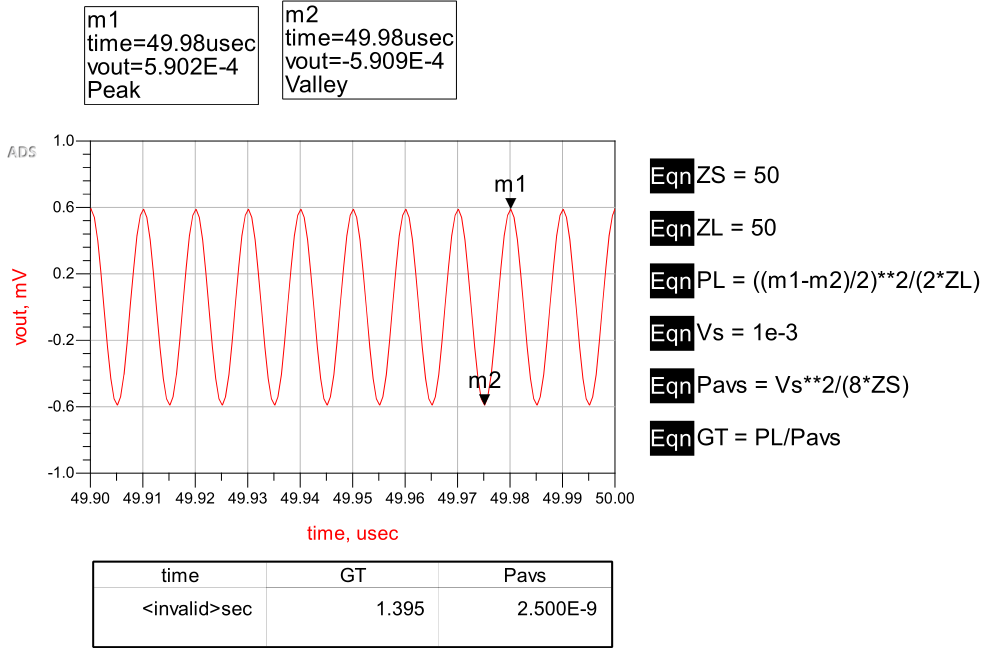
\includegraphics[width=13cm]{images/gtproof.png}
\caption{Proof of common-emitter amplifier with BC549 transducer power gain ($G_T$) at $100 MHz$.}
\label{p4:gtproof} 
\end{figure}

Another way to observe the transducer power gain is via a harmonic balance simulation at $100 MHz$. In this case it will not be used the circuit with the BJT, but a two ports generic quadripole characterized by the S-parameters founded before. The figure \ref{p4:Sparamcheck} show the SParamChecker for the generic quadripole of which the S-parameters sampled at $100 MHz$ matches the parameters obtained in the previous circuit like in figure \ref{p4:sparams}.

\begin{figure}[H] 
\centering
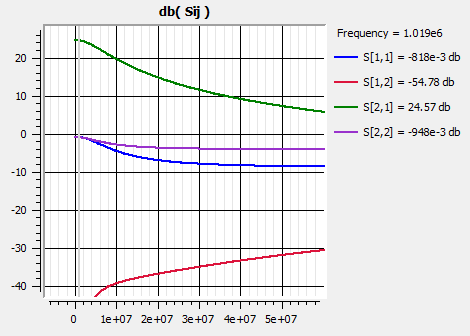
\includegraphics[width=9cm]{images/SParamChecker.png}
\caption{SParamChecker for generic quadripole.}
\label{p4:Sparamcheck} 
\end{figure}

Extracting the time domain signal from the load voltage in the harmonic balance (HB) simulation we observe the graphic in the figure \ref{p4:HB}. Despite feeding the quadripole with a $100 MHz$ sinusoidal voltage like in the previous simulation, the result for the transducer power gain differs from the previous simulations. 

\begin{figure}[H] 
\centering
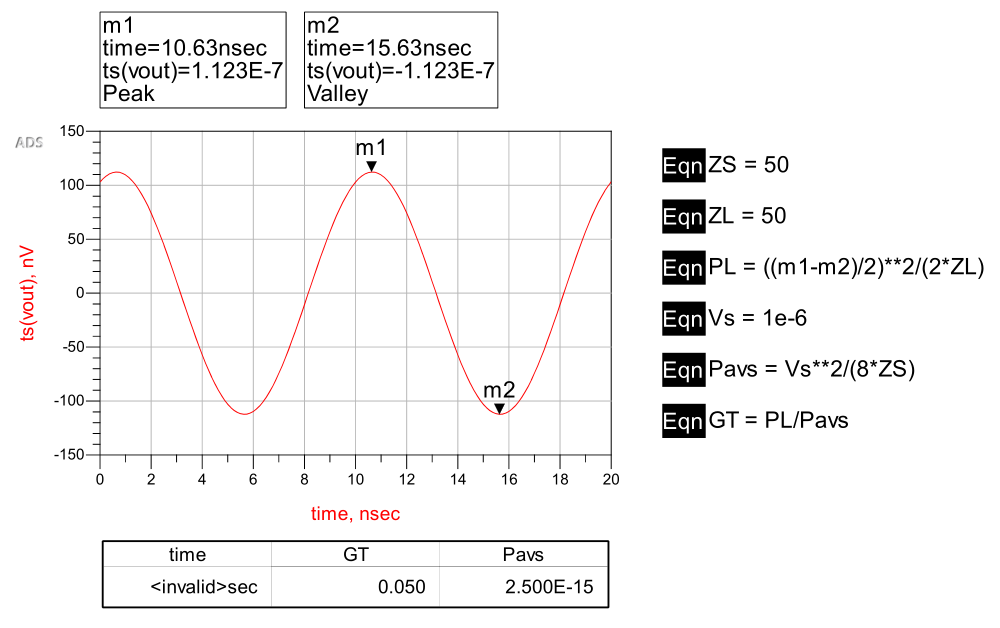
\includegraphics[width=12cm]{images/HB.png}
\caption{Time domain signal from HB simulation.}
\label{p4:HB} 
\end{figure}

This problem might have occurred due to maladjustments in the circuit parameters.